\documentclass[a4paper, 12pt, oneside]{scrbook}

\input{settings.tex}

\bibliography{bibliography.bib}
\begin{document}

\frontmatter

% Hierin müssen Matrikelnummer Name usw. gesetzt werden.
\input{prefix/title.tex}

\pagenumbering{gobble}
\input{prefix/eigenstaendigkeit.tex}

% Kurzfassung
\section*{Kurzfassung}
Diese Studienarbeit behandelt die Entwicklung einer Anwendung zum Verwalten von Schichtwechseln unter der Verwendung des Google Design Sprints. Zunächst wurde die UX entwickelt und anschließend darauf basierend ein Benutzerkonzept, um die Nutzerfreundlichkeit und Effektivität der Anwendung zu gewährleisten. Im Anschluss daran wurde eine Nutzerumfrage durchgeführt, um Feedback von den Anwendern zu sammeln. Diese Umfrage zielte darauf ab, herauszufinden, wie das Design bei den Nutzern ankommt, ob die Anwendung intuitiv ist und welche Verbesserungsvorschläge oder zusätzlichen Informationen von den Nutzern gewünscht werden. Die Ergebnisse der Umfrage wurden sorgfältig ausgewertet. Es stellte sich heraus, dass die Nutzer das Design im Allgemeinen gut fanden, jedoch einzeln Verbesserungsvorschläge und der Wunsch nach zusätzlichen Informationen geäußert wurde. Basierend auf diesen Erkenntnissen wurde das Benutzerkonzept überarbeitet, um besser auf die Bedürfnisse und Wünsche der Nutzer einzugehen. In der letzten Phase der Entwicklung wurde anhand des überarbeiteten Benutzerkonzepts ein Prototyp mit Angular erstellt. Diese dient als Grundlage für die weitere Entwicklung und Verfeinerung der Anwendung, um eine optimale Nutzererfahrung zu gewährleisten.

\clearpage

% Abstract
\section*{Abstract}

This student research project deals with the development of an application for managing shift changes using the Google Design Sprint. 
First, the UX was developed and then, based on this, a user concept was developed to ensure the user-friendliness and effectiveness of the application. 
Following this, a user survey was conducted to gather feedback from users. This survey aimed to find out how the design was received by users, whether the application was intuitive and what suggestions for improvement or additional information users would like to see. The results of the survey were carefully analyzed. It turned out that the users generally liked the design, but that there were individual suggestions for improvement and a request for additional information. Based on these results, the user concept was modified to better meet the needs and wishes of the users. In the final phase of development, a prototype was created with Angular based on the updated user concept. This serves as the basis for further development and refinement of the application to ensure an optimal user experience.

\tableofcontents

% Abbildungsverzeichnis
\cleardoublepage
\phantomsection
\addcontentsline{toc}{chapter}{\listfigurename}
\pagenumbering{Roman}
\listoffigures

% Tabellenverzeichnis
% \cleardoublepage
% \phantomsection
% \addcontentsline{toc}{chapter}{\listtablename}
% \listoftables

%Codebeispiel Verzeichnis
% \cleardoublepage
% \phantomsection
% \addcontentsline{toc}{chapter}{\lstlistlistingname}
% \lstlistoflistings

% Abkürzungsverzeichnis (siehe Ordner "content")
\chapter{Abkürzungsverzeichnis}
\begin{acronym}
    \acro{GDS}{Google Design Sprint}
    \acro{UX}{User Experience}
    \acro{TS}{TypeScript}
    \acro{JSON}{JavaScript Object Notation}
\end{acronym}

\mainmatter

%%%%%% Inhalt (siehe Ordner "content") %%%%%%
\input{content/Einleitung.tex}
\chapter{Grundlagen}

\section{Google Design Sprint}

Der \ac{GDS} ist eine von Jake Knapp bei Google Ventures entwickelte Methodik zur schnellen und effizienten Problemlösung sowie Produktentwicklung, insbesondere für Herausforderungen, die sich aus der dynamischen Natur des Marktes und den sich verändernden Produktanforderungen ergeben. 
Ziel dieser Methode ist es, innerhalb eines Zeitraums von fünf Tagen einen Prototyp zu entwickeln und zu evaluieren. 
Diese Methode bietet den Vorteil, dass nicht auf die Markteinführung gewartet werden muss, um Feedback zu erhalten. Stattdessen können dringende Fragen sofort beantwortet werden \cite[S.98 f.]{Design_Sprint}.

Die fünftägige Methode, wie in Abbildung \ref{GDS} dargestellt, verläuft wie folgt:

\begin{figure}[h]
    \centering
    \includegraphics[clip,width=0.75\linewidth]{images/GDS.png}
    \caption[Ablauf eines GDS]{Ablauf eines GDS \cite{GDS_Abbildung}}
    \label{GDS}
\end{figure}

Am ersten Tag geht es darum, das Problem zu verstehen und den Fokus für die Woche festzulegen. Das Team definiert das langfristige Ziel und identifiziert die Herausforderung. 

Am zweiten Tag konzentriert sich das Team auf die Bewältigung bereits bekannter Herausforderungen. Anders als bei herkömmlichen Brainstorming-Sitzungen arbeiten die Teammitglieder einzeln an Lösungsansätzen und folgen einem strukturierten vierstufigen Prozess, um das kritische Denken zu fördern. 

Am dritten Tag trifft das Team Entscheidungen darüber, welche Idee als Prototyp entwickelt und getestet werden sollen. Dabei kommt die fünfstufige „Sticky Decision“-Methode zum Einsatz, um die besten Lösungen zu identifizieren. Anschließend wird ein detaillierter Prozessplan für den Prototypen erstellt. 

Am vierten Tag wird ein realitätsnaher Prototyp entwickelt. Das Ziel ist es, eine testbare Version der Lösung zu erstellen, die am nächsten Tag mit echten Nutzern evaluiert werden kann. 

Der letzte Tag ist für das Testen des Prototyps reserviert. Das Team sammelt Feedback von echten Nutzern und erhält Einsicht, ob die Lösung in der Praxis funktioniert und welche Anpassungen nötig sind. Dieses Feedback ist entscheidend, um die Stärken und Schwächen der entwickelten Lösung zu identifizieren \cite[S.22 ff.]{Design_Sprint}.

\section{User Experience}
Das Design der \ac{UX} konzentriert sich auf jedes Element und jede Funktion, die der Benutzer bei einer Anwendung sieht, mit dem Ziel, eine möglichst angenehme und effiziente Erfahrung zu ermöglichen \cite[S.12]{Bordegoni}. 
Laut der International Organization for Standardization (ISO 9241-210) wird UX definiert als „Wahrnehmungen und Reaktionen einer Person, die sich aus der Verwendung und/oder der erwarteten Verwendung eines Produkts, Systems oder einer Dienstleistung ergeben” \cite{iso}. 
Während sich das User Interface auf das Erscheinungsbild der Anwendung konzentriert, beispielsweise auf Schriftarten und Farben, geht die UX tiefer und umfasst das gesamte Erlebnis des Nutzers \cite[S.8]{Canziba}.

In den letzten Jahrzehnten hat die Bedeutung der User Experience stark zugenommen, da Unternehmen erkannt haben, dass ein positives Nutzungserlebnis entscheidend für den Erfolg eines Produkts ist \cite{ux_article}. 
Bei einem schlechten UX-Design fällt es den Benutzern schwer, die Anwendung zu nutzen, und sie wechseln, sobald sie eine ähnliche, bessere App gefunden haben, die die gleiche Aufgabe erfüllt. 
Deshalb ist es für ein gutes UX-Design wichtig, dass der Designer die Bedürfnisse der Benutzer vorhersieht und erfüllt, indem er ihre Sichtweise einnimmt. Ein gutes UX-Design kann die Produktivität steigern, die Zufriedenheit der Kunden erhöhen und die Verkaufszahlen verbessern. 
Zudem können durch eine optimierte Benutzererfahrung die Kosten für Support und Wartung gesenkt werden \cite[S.8 ff.]{Canziba}.

Die UX umfasst verschiedene Komponenten, die zusammenarbeiten, um ein positives Nutzungserlebnis zu schaffen. Dazu gehören Usability, Ästhetik, Interaktion und Emotionalität.

Die Usability bezieht sich auf die Benutzerfreundlichkeit und Effizienz eines Produkts. 
Ein System mit hoher Usability ermöglicht es den Nutzern, ihre Ziele schnell und ohne Frustration zu erreichen. 
Dies beinhaltet Aspekte wie Lernfähigkeit, Effizienz der Nutzung und Zufriedenheit der Nutzer \cite[S.23 ff.]{Nielsen}.

Die Ästhetik bezieht sich auf das Erscheinungsbild des Produkts. 
Ein ansprechendes visuelles Design kann die Wahrnehmung der Qualität und den Gesamteindruck eines Produkts erheblich verbessern. 
Studien zeigen, dass ästhetisch ansprechende Designs oft als funktionaler und benutzerfreundlicher wahrgenommen werden \cite{Tractinsky}.

Die Interaktion beschreibt, wie Nutzer mit einem Produkt oder einer Dienstleistung umgehen. 
Dies umfasst die Art und Weise, wie Eingaben getätigt werden, wie das System auf Nutzeraktionen reagiert und wie intuitiv diese Interaktionen gestaltet sind. 
Gute Interaktionsdesigns minimieren die kognitive Belastung und fördern eine reibungslose und intuitive Nutzung \cite{interaction_design}.

Emotionalität in der UX bezieht sich auf die emotionalen Reaktionen und das subjektive Erleben der Nutzer während der Interaktion mit einem Produkt. 
Positive emotionale Erfahrungen können die Benutzerbindung und Zufriedenheit erhöhen. 
Studien belegen, dass Produkte, die positive Emotionen hervorrufen, häufiger genutzt und weiterempfohlen werden \cite{emotion}.

Es gibt eine Vielzahl von Methoden zur Bewertung der UX, zu den gebräuchlichsten Methoden gehören:

Usability-Tests beinhalten die Beobachtung und Analyse der Nutzerinteraktionen mit einem System, um Nutzerprobleme zu identifizieren. 
Durch das Testen in realistischen Nutzungsszenarien können konkrete Probleme und deren Schweregrad ermittelt werden, was zur Verbesserung der Nutzerfreundlichkeit beiträgt. 
Diese Methode ist besonders effektiv, um zu verstehen, wie Nutzer tatsächlich mit dem System interagieren \cite[S.165 ff.]{Nielsen}.

Mit Nutzerbefragungen und Interviews können qualitative Daten direkt von den Nutzern gesammelt werden. 
Diese Methode ermöglicht es, tiefergehende Einblicke in die Meinungen, Erfahrungen und Verbesserungsvorschläge der Nutzer zu gewinnen, was zur Optimierung der Interaktionen und der allgemeinen Zufriedenheit beitragen kann. 
Durch gezielte Fragen können spezifische Aspekte der Nutzererfahrung identifiziert und adressiert werden \cite{ux_bewertung_interview}.

Bei der Eye-Tracking-Technologie wird die Augenbewegungen von Nutzern verfolgt, wie in Abbildung \ref{eye_tracking} dargestellt. 

\begin{figure}[h]
    \centering
    \includegraphics[clip,width=0.4\linewidth]{images/Eye-Tracking-Google-Search-Heat-Map.jpg}
    \caption[Beispielhafte Visualisierung der Eye Tracking Methode anhand einer Heat Map]{Beispielhafte Visualisierung der Eye Tracking Methode anhand einer Heat Map \cite{image_eye_tracking}}
    \label{eye_tracking}
\end{figure}

Durch die Messung von Fixationen, also den Momenten, in denen das Auge auf einem Punkt verharrt, kann festgestellt werden, welche Elemente einer Benutzeroberfläche besondere Aufmerksamkeit erregen. 
Sakkaden, die schnellen Augenbewegungen zwischen Fixationen, helfen dabei zu verstehen, wie Nutzer Informationen auf einer Seite scannen. 
Diese Daten liefern wertvolle Einblicke in die Nutzerinteraktion und ermöglichen die Optimierung von Design und Layout basierend auf tatsächlichen Nutzerverhalten \cite[S.3 ff.]{eye_tracking}.
  
Durch die Kombination dieser Methoden können umfassende Einblicke in die Stärken und Schwächen der User Experience gewonnen werden, die zur kontinuierlichen Verbesserung des Produkts beitragen.

\section{Technologien}

\subsection{Das Angular-Framework}
Angular ist eine Plattform zur Entwicklung von Webanwendungen, die auf \ac{TS} basiert. 
Mit Angular können Single Page Applications für Web-, Mobil- und Desktop-Anwendungen entwickelt werden. 
Es ist Open Source und wird von Google unterstützt, was bedeutet, dass es kostenlos verwendet werden kann und von einer großen Entwickler-Community gepflegt wird. 
Ursprünglich war es als AngularJS bekannt und nutzte JavaScript als Hauptprogrammiersprache. Die Codebasis wurde jedoch komplett neu geschrieben, wobei JavaScript durch TS ersetzt wurde \cite{angular_arch}.

\begin{figure}[h]
    \centering
    \includegraphics[clip,width=0.5\linewidth]{images/Komponente.png}
    \caption[Komponenten in Angular]{Komponenten in Angular}
    \label{KomponentenAngular}
\end{figure}

Die grundlegenden Bausteine des Angular-Frameworks sind die Komponenten, welche eine isolierte und somit wieder verwendbar Einheit sind. 
Eine Komponente besteht aus einer HTML- und CSS-Datei (siehe Abbildung \ref{KomponentenAngular}), die das Aussehen der Benutzeroberfläche definieren. Die zugehörige Klasse enthält den TS Code, der das Verhalten der Komponente steuert \cite{angular_arch}.

\begin{figure}[h]
    \centering
    \includegraphics[clip,width=0.5\linewidth]{images/@Component.png}
    \caption[@Component-Dekorator in TypeScript]{@Component-Dekorator in TS}
    \label{Component}
\end{figure}

Der @Component-Dekorator in TS fügt der Klasse zusätzliche Metadaten hinzu, wie den Pfad zum Template und zu den Styles (siehe templateUrl und styleUrls in der Abbildung \ref{Component}) \cite{angular_arch}.

Durch Unit-Tests in Angular ist es möglich, isoliert einzelne Teile der Anwendung zu testen, um sicherzustellen, dass diese gemäß den Erwartungen funktionieren. 
Diese Tests sind in .spec.ts Dateien organisiert und umfassen Testfälle für Komponenten, Dienste und Module. 
Sie werden üblicherweise mit Testing-Frameworks wie Jasmine und Karma ausgeführt, die in die Angular-Entwicklungsumgebung integriert sind. 
Neben Unit-Tests gibt es auch End-to-End-Tests, die das Verhalten der Anwendung in einer realen Umgebung simulieren \cite[S.340 ff.]{angular_testing}.

Der Routing-Service ermöglicht es verschiedene Ansichten basierend auf der URL der Anwendung zu laden. 
Durch die Definition von Routen und deren Zuordnung zu spezifischen Komponenten ermöglicht Angular eine klare Strukturierung und Navigation innerhalb der Anwendung, was insbesondere für komplexe Single Page Applications entscheidend ist. 
Routen können parameterisiert werden oder der Zugriff auf bestimmte Routen kann durch Guards gesteuert werden \cite{angular_routes}.

\subsection{MongoDB}
MongoDB ist eine dokumentenorientierte NoSQL-Datenbank und entstand 2007 aus einem Platform-as-a-Service-Projekt von dem Start Up 10gen, das auf automatisiertes Infrastrukturmanagement abzielte. 
Aufgrund der Ablehnung durch Entwickler, die Kontrolle über ihre Technologie-Stacks zu verlieren, fokussierte sich 10gen auf die Datenbank und benannte sich in MongoDB, Inc. um. 
MongoDB wird als Open-Source-Projekt entwickelt, wobei die Community zur Mitarbeit ermutigt wird, das Geschäftsmodell umfasst die Unterstützung der Open-Source-Entwicklung und das Anbieten von Abonnementdiensten \cite[S.5 f.]{Banker2016MongoDB}.

MongoDB wurde zur schnellen Entwicklung von Webanwendungen und Internet-Infrastruktur designed. 
Es ist möglich, ein strukturiertes Dokument in der Datenbank zu speichern, ohne bei der Erstellung der Datenbank schon wissen zu müssen, wie die Datenstruktur aussehen wird oder neue Tabellen erstellen zu müssen, wenn sich die Daten ändern. 
Die Struktur wird durch den Code der Anwendung bestimmt. Außerdem ist es, wenn für die Speicherung der Datenmenge mehr als eine Datenbank benötigt wird, mit MongoDB deutlich einfacher und performante diese zu skalieren, als bei einer relationalen Datenbank \cite[S.4 ff.]{Banker2016MongoDB}. 

Intern speichert MongoDB die Daten als Binary \ac{JSON}, eine Struktur, die JSON ähnelt, jedoch für die Speicherung vieler Dokumente optimiert ist. 
Nach einer Abfrage werden die Ergebnisse in eine leicht lesbare Datenstruktur übersetzt, das Dokumentenformat JSON, das aus Schlüsseln und Werten besteht (für Beispiel siehe Abbildung \ref{MongoDB_Document}). 
Während relationale Datenbanken Tabellen verwenden, nutzt MongoDB stattdessen Kollektionen \cite[S.7]{Banker2016MongoDB}.

\begin{figure}[h]
    \centering
    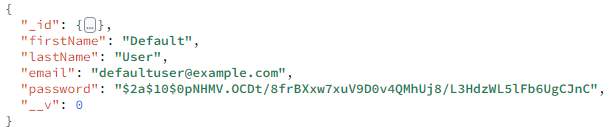
\includegraphics[clip,width=0.65\linewidth]{images/MongoDB_Document.png}
    \caption[Beispiel eines Dokuments in einer MongoDB]{Beispiel eines Dokuments in einer MongoDB}
    \label{MongoDB_Document}
\end{figure}

Insgesamt bietet MongoDB eine leistungsfähige, flexible und skalierbare Lösung für die Verwaltung komplexer und dynamischer Datenmodelle, was sie ideal für moderne Webanwendungen macht.

\subsection{Node.js}
Node.js ist eine serverseitige Laufzeitumgebung, die auf der V8-JavaScript-Engine von Google Chrome basiert und die Ausführung von JavaScript-Code außerhalb des Browsers ermöglicht. 
Entwickelt von Ryan Dahl im Jahr 2009, hat sich Node.js schnell als leistungsfähige Plattform für die Erstellung von serverseitigen Anwendungen etabliert \cite[S.3 ff.]{Cantelon2014}. 
Ein wesentliches Merkmal von Node.js ist sein ereignisgesteuertes, nicht-blockierendes I/O-Modell, das eine effiziente Verarbeitung gleichzeitiger Verbindungen ermöglicht \cite{Tilkov2010}. 
Diese Architektur ist besonders für Anwendungen geeignet, die häufige I/O-Operationen ausführen, wie beispielsweise APIs oder kleine Webserver. 
Ein weiterer Vorteil von Node.js ist die Nutzung von JavaScript sowohl auf der Client- als auch auf der Serverseite, was zu einer einheitlichen Codebasis und vereinfachten Entwicklungsprozessen führt . 
Die Kombination von Angular und Node.js bietet daher eine schnelle und effiziente Datenverarbeitung sowie eine einheitliche Entwicklungsumgebung \cite[S.5 ff.]{Casciaro2020node}.
\chapter{Entwicklung der User Experience mit Verwendung des Google Design Sprints}

Die Entwicklung eines nutzerfreundlichen und effektiven UX-Design-Konzepts zur Abstimmung von Schichtwechseln wurde mithilfe des GDS realisiert. Ursprünglich wurde der GDS für einen Zeitraum von fünf Tagen entwickelt, um schnell Lösungen für komplexe Probleme zu finden und neue Ideen zu testen. In diesem Projekt wurde der GDS aufgrund der Durchführung durch eine Einzelperson angepasst.

Die Phasen 4 und 5 des GDS, die normalerweise die Entwicklung eines Prototypen und das Testen umfassen, wurden modifiziert. Stattdessen wurde ein umfangreiches Bedienungskonzept entwickelt, auf dessen Grundlage eine Nutzerumfrage durchgeführt wurde (siehe Kapitel~\ref{chap:nutzerumfrage}) .
Die Ergebnisse dieser Umfrage wurden anschließend genutzt, um das Benutzerkonzept weiter zu verbessern und anschließend den Prototypen zu erstellen.

\section{Phase 1: Verstehen und Definieren}
In der ersten Phase werden die benötigten Informationen gesammelt und analysiert, um das Problem umfassend zu verstehen und klar zu definieren. Die Problemstellung und Zielsetzung wurden bereits in der Einleitung ausführlich behandelt, daher wird in diesem Kapitel direkt auf die praktische Anwendung der nächsten Phasen eingegangen.

\section{Phase 2 und 3: Skizzieren und Auswahl der Idee}
In der Skizzieren Phase beginnt der Prozess der Designerstellung. Hierbei wurden sich zunächst die benötigten Seiten überlegt, um die benötigten Aufgaben und Anforderungen zu erfüllen. Dazu gehört eine Übersichtsseite auf der alle aktuellen Tauschangebote stehen und worüber der Nutzer zu allen weiteren Seiten gelangt, z.B. die zum Hinzufügen und zum Annehmen eines Tauschangebots, sowie eine Seite, auf der der Nutzer seine angenommen Schichten sehen kann und individuelle Einstellungen vornehmen kann. 

Die erste Version der Übersichtsseite war zunächst für einen Desktop ausgelegt (siehe Abbildung \ref{Version1_Desktop}). 

\begin{figure}[h]
    \centering
    \includegraphics[clip,width=1\linewidth]{images/Version1_Desktop.png}
    \caption[Erste Version der Übersichtsseite für den Desktop]{Erste Version der Übersichtsseite für den Desktop}
    \label{Version1_Desktop}
\end{figure}

Im oberen Bereich der Seite befindet sich der Header. 
Links darunter hat der Nutzer die Möglichkeit zwischen den Monaten zu navigieren. 
Rechts unter dem Header befindet sich „Neues Tauschangebot erstellen“ Button, mit dem Nutzer neue Tauschangebote erstellen können. 
Zentral auf der Seite ist der Kalender des aktuellen Monats groß dargestellt, die Wochentage sind darüber ausgeschrieben.

Bei der Übertragung des Designs in die Handy-Version wurden einige Schwachstellen identifiziert. Die Darstellung des Desktop-Designs auf dem Handy führt dazu, dass die Schrift aufgrund der kleinen Größe schlecht lesbar war (siehe Abbildung \ref{Version12_Handy}). 

\begin{figure}[h]
    \centering
    \includegraphics[clip,width=0.75\linewidth]{images/Version12_Handy.png}
    \caption[Erste und zweite Version der Übersichtsseite für das Handy]{Erste und zweite Version der Übersichtsseite für das Handy}
    \label{Version12_Handy}
\end{figure}

Da die meisten Nutzer die App wahrscheinlich auf dem Handy verwenden möchten, wurde das Design in Version 2 entsprechend angepasst.

Um in der Kalenderübersicht die Tauschanfragen gut lesbar und nutzerfreundlich darzustellen, werden statt fünf Wochen nur noch zwei Wochen angezeigt (siehe Version 2 in Abbildung \ref{Version12_Handy}). 
Aufgrund der schmaleren Handybildschirme wird ein Teil der Wörter durch Piktogramme ersetzt, z.B. wurde beim „Neues Tauschangebot erstellen“ Button der Text durch ein Plus ersetzt. Dadurch wird Platz gespart und die Funktion wird klarer erkannt. 
Außerdem werden die Wochentage nicht mehr ausgeschrieben. Eine weitere Änderung ist, dass die Schichten in den gesuchten/gebotenen Zeit Blöcken am Tag abgebildet (siehe Version 2 in Abbildung \ref{Version12_Handy}).

Allerdings wurde festgestellt, dass der Kalender unübersichtlich wird, wenn mehrere Tauschangebote an einem Tag sind oder wenn welche zum gleichen Zeitpunkt angefragt werden. 
Deswegen wird eine weitere Version erstellt, in der die Schichten nicht mehr nach dem Zeitpunkt sortiert sind, sondern in einem Block organisiert, was eine bessere Übersicht ermöglicht (siehe Abbildung \ref{Version3_Handy}).

\begin{figure}[h]
    \centering
    \includegraphics[clip,width=0.75\linewidth]{images/Version3_Handy.png}
    \caption[Dritte Version der Übersichtsseite für das Handy, im Light Mode und Dark Mode]{Dritte Version der Übersichtsseite für das Handy, im Light Mode und Dark Mode}
    \label{Version3_Handy}
\end{figure}

Des weiteren wurde die Hauptfarbe von einem hellen Blau zu einem Orange gewechselt, welches wärmer und aktiver wirkt. Da der Dark Mode in den letzten Jahren stark an Popularität zugenommen hat \cite{diva2020darkmode} wird für die Anwendung auch ein Farbkonzept erstellt (siehe Dark Mode in Abbildung \ref{Version3_Handy}). 

Für die dritte Version wurde sich letztendlich entschieden. Darauf aufbauend wurden die weiteren Seiten der Anwendung im Light Mode gestaltet.

\section{Phase 4: Entwicklung des Bedienungskonzepts}
\label{sec:bedienungskonzept}
Um den Nutzern eine bessere Vorstellung von der UX zu vermitteln, wurden zwei unterschiedliche Farbpaletten erstellt: eine für den Light Mode und eine für den Dark Mode (siehe Abbildung \ref{Farbpalette}).

\begin{figure}[h]
    \centering
    \includegraphics[clip,width=0.9\linewidth]{images/Farbpalette.png}
    \caption[Farbpalette für den Light Mode und Dark Mode]{Farbpalette für den Light Mode und Dark Mode}
    \label{Farbpalette}
\end{figure}

Die Farbpalette für den Light Mode besteht aus verschiedenen Orangetönen und einem Braun. Die Hintergrundfarbe des Dark Modes ist ein dunkles Blau, Orange wird nur noch als Akzentfarbe verwendet, ansonsten wird ein helleres Blau genutzt.
Die Schriftart „Aptos“ wurde aufgrund ihrer Lesbarkeit und Ästhetik ausgewählt.

Ein zentrales Element des UX Designs war die Entwicklung eines klaren und intuitiven Bedienungskonzepts. Ziel war es, eine benutzerfreundliche Navigation zu schaffen, die es den Nutzern ermöglicht, alle Funktionen der Anwendung schnell und einfach zu erreichen.

\begin{figure}[h]
    \centering
    \includegraphics[clip,width=1\linewidth]{images/Bedienungskonzept_V1.png}
    \caption[Bedienungskonzept der Anwendung]{Bedienungskonzept der Anwendung}
    \label{Bedienungskonzept_V1}
\end{figure}

Nachdem sich der Nutzer registriert und anschließend erfolgreich angemeldet hat, gelangt er auf die zentrale Übersichtsseite, wie in Abbildung \ref{Bedienungskonzept_V1} dargestellt. 
Diese ermöglicht den Zugang zu allen anderen Seiten der Anwendung. 
Über die User-Kennung im Header gelangt der Nutzer zu einer Einstellungsseite. 
Dort kann er seine persönlichen Daten ändern und die bereits getauschten Schichten einsehen. 
Durch Klicken auf den Namen der Anwendung „Schichtentauschbörse“ im Header gelangt er jederzeit zurück zur Übersicht.

Möchte ein Nutzer eine neue Tauschanfrage erstellen, ist das über den Button direkt unter dem Header möglich. 
Dabei wird eine neue Seite aufgerufen, auf der die gebotene und gesuchte Schicht aus einem Dropdown-Menü ausgewählt werden können. 
Alternativ kann der Nutzer auch eine bestimmte Uhrzeit eingeben, falls eine spezifische Zeit gewünscht ist. 
Wenn der Nutzer seine Anfrage doch nicht stellen möchte, kann er den Vorgang abbrechen und gelangt zurück zur Übersichtsseite. 
Mit dem Drücken des „Erstellen“-Buttons wird die neue Tauschanfrage finalisiert und im Kalender für alle Nutzer sichtbar.

Klickt ein Nutzer im Kalender auf eine Anfrage, kann er das Annehmen der Tauschanfrage entweder über den Button „Abbrechen“ beenden oder über den Button „Tauschen“ die Schicht tauschen. 
Nach dem Annehmen verschwindet die Tauschanfrage aus dem Kalender und wird in den Einstellungen unter „Meine getauschten Schichten“ angezeigt.

Zusätzlich wurde eine alternative Dark Mode-Version der Übersichtsseite erstellt, um unterschiedliche Präferenzen der Nutzer einzubinden.

\section{Phase 5: Nutzerumfrage}
\label{chap:nutzerumfrage}
Die Farbpalette und die Übersicht über das Bedienungskonzept, für detailliertere Informationen siehe Abschnitt~\ref{sec:bedienungskonzept}, bilden die Grundlage für die Nutzerumfrage. Diese wurde als zentraler Bestandteil der Evaluierung des UX Designs der Webanwendung durchgeführt. Ziel der Umfrage ist es, Feedback von den Nutzern zu sammeln, um die Benutzerfreundlichkeit und Zufriedenheit zu messen und mögliche Verbesserungspotenziale zu identifizieren.

Die Umfrage richtete sich an die zukünftigen Endnutzer der Schichttauschanwendung innerhalb der Firma. Für detailliertere Informationen zum Fragebogen der Nutzerumfrage, siehe Anhang~\ref{app:fragebogenNutzerumfrage}.

\subsection{Methodik und Durchführung der Nutzerumfrage}

Die Umfrage besteht aus einem einem quantitativen und einem qualitativen Abschnitt. Der quantitative Teil der Umfrage umfasst Fragen, die die Intuitivität der Funktionen, die Ansprechbarkeit des visuellen Designs, die Übersichtlichkeit des Bildschirmaufbaus, die Ästhetik im Light Mode und Dark Mode sowie die Präferenz für die Nutzung der Anwendung über Web, Handy oder beides bewertet haben.

Im qualitativen Teil der Umfrage wurden die Teilnehmer durch offene Fragen dazu angeregt, ihre Verbesserungsvorschläge und Anregungen zur Umsetzung zu geben. Es wurde nach den fehlenden Funktionen oder Informationen sowie den wichtigsten Aspekten für die Nutzer gefragt.

Die Umfrage wurde online über ein Microsoft Forms Dokument durchgeführt, was eine einfache Verteilung und Teilnahme ermöglicht hat.

\subsection{Auswertung und Analyse der Nutzerumfrage}

An der Umfrage haben fünf von sechs zukünftigen Nutzern der Schichttauschanwendung teilgenommen. Die Ergebnisse bieten einen Einblick in die Benutzerfreundlichkeit, das visuelle Design und die Funktionalität der Anwendung.

Die Teilnehmer bewerteten die Intuitivität der Funktionen der Anwendung durchschnittlich mit 9,0 von 10 Punkten. Dies deutet darauf hin, dass die meisten Nutzer die Bedienung der Anwendung als sehr intuitiv empfanden. Dennoch wurden spezifische Verbesserungswünsche geäußert, es wurde der Wunsch geäußert, den Prozess des Ringtausches zu erleichtern und klare Kommunikationsmöglichkeiten bei der Angabe von Schichten zu schaffen, die für den Tausch angeboten werden können, insbesondere wenn ein Nutzer nur nach einer späteren Schicht sucht.

Die Umfrageergebnisse der wichtigsten Aspekte für den Nutzer zeigen, dass diesen vor allem die Übersichtlichkeit der Anwendung am wichtigsten ist, was fünfmal genannt wurde. Weitere bedeutende Aspekte umfassen die Effizienz der Anwendung, die Organisation bei mehreren Tauschwünschen an einem Tag und die Bestätigung des Tauschs mit möglichst wenigen Schritten. Außerdem wurde der Wunsch nach helleren Farben für einen besseren Kontrastmodus und ein schnelles Erfassen der gesuchten Schichten geäußert.

Das visuelle Design der Anwendung wurde im Durchschnitt mit 7,2 Punkten bewertet. 

\begin{figure}[h]
    \centering
    \includegraphics[clip,width=0.65\linewidth]{images/Grafik_Umfrage_visuelles_Design.png}
    \caption[Bewertung des visuellen Designs der Anwendung]{Bewertung des visuellen Designs der Anwendung}
    \label{Grafik}
\end{figure}

Wie in Abbildung \ref{Grafik} dargestellt, reichten die Bewertungen von 3 bis 9 Punkten, was auf eine unterschiedliche Wahrnehmung und verschiedene Präferenzen der Nutzer hinweist.

Die Übersichtlichkeit des Bildschirmaufbaus erhielt eine sehr hohe durchschnittliche Bewertung von 9,4 Punkten. Dies zeigt, dass die Mehrheit der Nutzer den Bildschirmaufbau als sehr klar und strukturiert empfand.

Die allgemeine Ästhetik der Anwendung wurde sowohl im Light Mode als auch im Dark Mode bewertet. Der Light Mode erhielt eine durchschnittliche Bewertung von 8,0 Punkten, während der Dark Mode eine durchschnittliche Bewertung von 6,8 Punkten erhielt. Zwei Personen gaben an, dass ihnen der Light Mode deutlich besser gefiel (3 bzw. 4 Punkte Unterschied), während zwei andere Personen den Dark Mode bevorzugten (2 und 1 Punkt Unterschied). Eine Person bewertete beide Modi gleich gut.

Die Mehrheit der Nutzer (vier von fünf) gab an, hauptsächlich die mobile App nutzen zu wollen, während eine Person sowohl die Web-Anwendung als auch die mobile App gleich häufig nutzen würde. Dies bestätigt die beim Entwurf der Anwendung getroffene Vermutung.

Die Nutzer äußerten mehrere Vorschläge für zusätzliche Informationen und Funktionen, die das Tauschen der Schichten vereinfachen könnten. Dazu gehören:

\begin{itemize}
    \item Eine Anzeige, ob an einem Dienst ein Trainee beteiligt ist.
    \item Die Möglichkeit, Anfragen als dringend zu kennzeichnen.
    \item Ein Feld für Details zu den Anfragen.
    \item Eine Priorisierung bei mehreren Personen, die die gleiche Schicht suchen.
    \item Eine Verknüpfung mit dem eigenen Kalender, um Tauschmöglichkeiten schnell zu erkennen.
    \item Die Anzeige aller möglichen Tauschpartner und der zu tauschenden Dienste.
    \item Ideal wäre eine Anbindung an den Kalender oder den tatsächlichen Dienstplan, um das Hin- und Herspringen zwischen Anwendungen zu vermeiden.
  \end{itemize}

Alle Teilnehmer gaben an, dass die Anwendung ihren Anforderungen entspricht, abgesehen von den Anmerkungen bei den vorherigen Fragen. Dies zeigt, dass die Anwendung bereits viele Bedürfnisse der Nutzer erfüllt, jedoch weiterhin etwas Raum für Verbesserungen und die Integration zusätzlicher Informationen besteht.
\input{content/neues_Bedienungskonzept.tex}
\chapter{Entwicklung eines Prototypen des Benutzerkonzepts mit dem Angular-Framework}
\label{chap:prototyp}
Der Prototyp ist auf Basis des vorher entwickelten Benutzerkonzepts entwickelt. Für eine genaue Beschreibung des Benutzerkonzepts siehe Abschnitt~\ref{sec:bedienungskonzept}.

\section{Backend}
Das Backend ist mit Node.js und MongoDB entwickelt. 
Hierbei wird der Express-Server von Node.js und die Mongoose-Bibliothek von MongoDB verwendet, um eine effiziente und skalierbare Datenverwaltung zu gewährleisten.

Die Kernfunktionalitäten des Backends umfassen die Benutzerregistrierung und -verwaltung. 
In der Datei \texttt{server.js} werden die Endpunkte für die Registrierung und Anmeldung der Nutzer definiert. 
Die Datei \texttt{userModel.js} enthält das Schema für die Benutzer, welches die Felder Vorname, Nachname, E-Mail-Adresse und Passwort umfasst. 
Das Passwort wird in der \texttt{userModel.js}-Datei mithilfe der Bibliothek bcryptjs verschlüsselt, bevor es in der Datenbank gespeichert wird. 
Dies stellt sicher, dass Passwörter nicht im Klartext in der Datenbank gespeichert werden. 
 Datei \texttt{server.js} ist ebenfalls für die Überprüfung zuständig, ob ein Nutzer existiert und ob seine Anmeldedaten korrekt sind. 
 Dies ermöglicht eine sichere Authentifizierung der Nutzer.

Die Registrierung eines neuen Nutzers erfolgt über die Methode \texttt{app.post('/api/register', async (req, res) => \{ ... \})}. 
Der Nutzer gibt seine Daten ein, und bei korrekter Eingabe wird ein neues Benutzerobjekt basierend auf diesen Eingaben erstellt. 
Über die Methode \texttt{app.post('/api/login', async (req, res) => \{ ... \})} wird beim Anmeldeversuch eines Nutzer abgeglichen, ob die eingegebenen E-Mail-Adresse und das Passwort mit den in der Datenbank gespeicherten Daten übereinstimmen. 
Zunächst wird überprüft, ob ein Nutzer mit der angegebenen E-Mail-Adresse existiert. 
Falls nicht, wird eine Fehlermeldung „Benutzer nicht gefunden“ zurückgegeben. 
Anschließend wird das eingegebene Passwort mit dem in der Datenbank gehashten Passwort verglichen. 
Ist das Passwort falsch, erhält der Nutzer die Fehlermeldung „Falsches Passwort“. 
Bei korrekter Eingabe der Anmeldedaten wird die Nachricht „Login erfolgreich“ zurückgegeben.

\section{Frontend}
Das Frontend der Anwendung ist mit dem Angular Framework entwickelt. 
Alle Seiten der Anwendung sind responsiv gestaltet, sodass die Nutzer die Anwendung sowohl auf dem Handy als auch auf dem Laptop angenehm nutzen können. 
Für den Dark Mode werden derzeit die Systemeinstellungen des Geräts verwendet.

\begin{figure}[h]
    \centering
    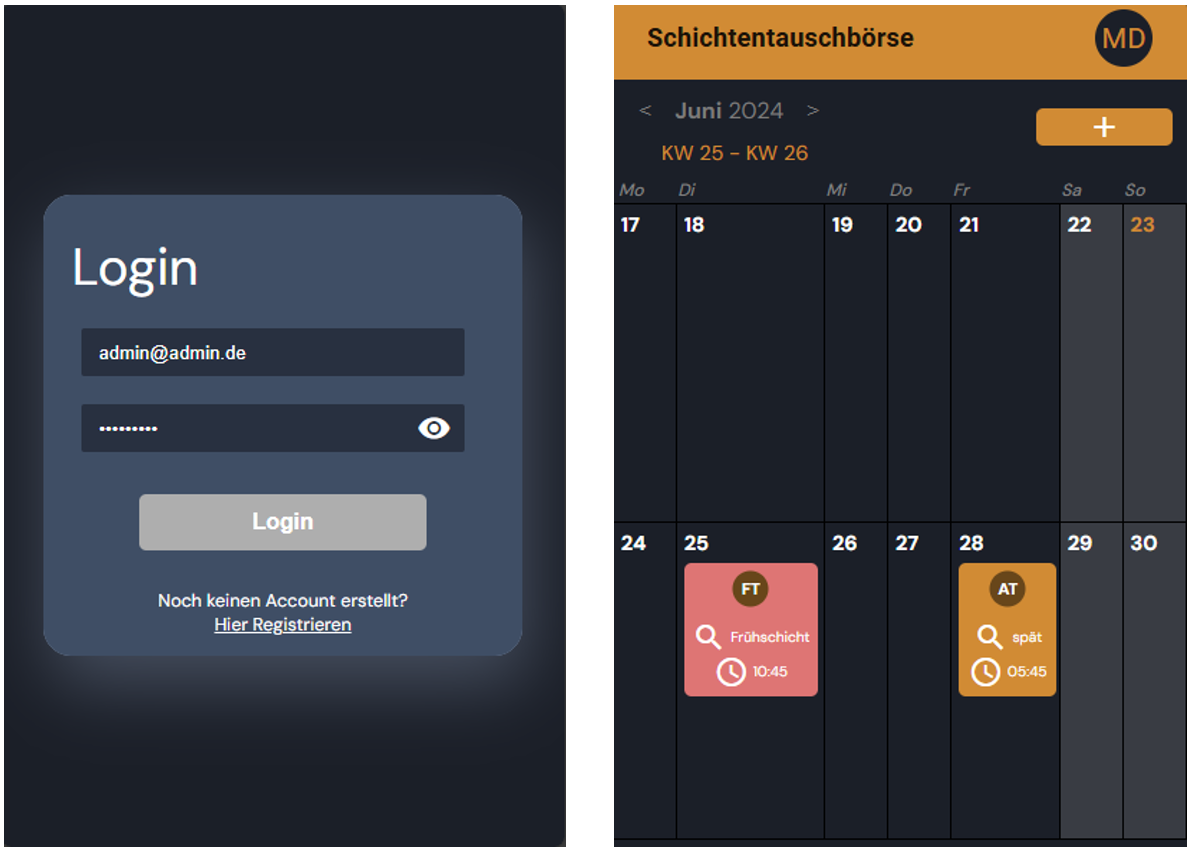
\includegraphics[clip,width=0.8\linewidth]{images/Login_Home_dark.png}
    \caption[Login- und Übersichtsseite im Dark Mode auf einem 400x600px großen Bildschirm]{Login- und Übersichtsseite im Dark Mode auf einem 400x600px großen Bildschirm}
    \label{Login_Home_dark}
\end{figure}

Wenn ein Nutzer die Anwendung zum ersten Mal benutzt, muss er sich zunächst registrieren. 
Die Eingabefelder für die Registrierung werden validiert, um sicherzustellen, dass beispielsweise die E-Mail-Adresse im richtigen Format eingegeben wird. 
Mit der \texttt{PasswordStrengthValidator()} Funktion wird überprüft, ob das Passwort sicher genug ist. 
Da der Nutzer das Passwort zur Überprüfung zweimal eingeben muss, wird mithilfe der \texttt{passwordMatchValidator()} Funktion sichergestellt, dass beide Passwörter übereinstimmen. 
Falls dies nicht der Fall ist, wird eine Fehlermeldung angezeigt. 
Über das Augensymbol im Eingabefeld kann der Nutzer sich jedoch seine Passwörter anzeigen lassen (siehe Login-Seite in Abbildung \ref{Login_Home_dark}).

Der Service \texttt{user.service.ts} kommuniziert für Login und Registrierung über HTTP-Anfragen mit dem Express-Server im Backend. 
Nach erfolgreicher Registrierung wird der Nutzer zum Login-Formular weitergeleitet, wo er sich mit seinem erstellten Account anmelden kann. 
Wenn die Anmeldedaten korrekt sind, wird der Nutzer zur Übersichtsseite weitergeleitet, von der aus alle anderen Seiten erreichbar sind.

Die Felder, in denen ein Tauschangebot eingetragen ist, sind etwas breiter, damit die Informationen besser zu erkennen sind. 
Der heutige Tag ist farbig hervorgehoben, wie in Abbildung \ref{Login_Home_dark} zu sehen ist.

Zusätzlich kann sich der Nutzer in den Einstellungen auch wieder ausloggen. Hierfür wird die Funktion \texttt{logout()} aus der \texttt{auth.service.ts}-Datei verwendet. 
Eine Funktion zum Exportieren der Tauschangebote in den Kalender wird im Frontend bereits angezeigt, ist jedoch im Backend noch nicht implementiert.

Wenn der Nutzer auf der Übersichtsseite auf den Button mit dem Plus klickt, kann er eine neue Tauschanfrage erstellen, die Eingabefelder dafür verwenden Angular Material. 
Der Nutzer kann das Datum aus einem Kalender auswählen oder selbst eingeben. Die angebotene und gesuchte Schicht kann aus einem Dropdown-Menü ausgewählt werden. 
Wenn der Nutzer eine benutzerdefinierte Uhrzeit eingeben möchte, kann er "Benutzerdefinierte Uhrzeit" auswählen. 
Dann erscheint ein neues Eingabefeld, in dem er diese Uhrzeit eintragen kann. Durch Angular Material wird sichergestellt, dass die Uhrzeit im richtigen Format eingegeben wird. 
Eine Anfrage kann nur abgeschickt werden, wenn mindestens das Datum sowie die angebotene und gesuchte Schicht eingetragen sind.

Durch Klicken auf ein Tauschangebot im Kalender (siehe Abbildung \ref{Login_Home_dark}) öffnet sich eine Seite mit detaillierteren Informationen, je nachdem, welche Informationen für die Schicht relevant sind und vom Nutzer eingetragen wurden.
\chapter{Fazit und Ausblick}

Die manuelle Methode zur Verwaltung von Schichtwechseln über WhatsApp hat Herausforderungen und Ineffizienzen aufgezeigt. Die ständige Aktualisierung der Liste führt zu einer unübersichtlichen Informationsflut, wodurch Änderungen oder neue Einträge leicht übersehen werden können.

Durch die Anwendung des GDS konnte eine effizientere und nutzerfreundlichere Lösung zur Abstimmung von Schichtwechseln entwickelt werden. In diesem Projekt wurde der GDS an die Durchführung durch eine Einzelperson angepasst, wobei die Phasen 4 und 5 modifiziert wurden, um ein umfangreiches Bedienungskonzept zu entwickeln und anschließend daran eine Nutzerumfrage durchzuführen.

Die Nutzerumfrage, die als zentraler Bestandteil der Evaluierung des UX-Designs diente, zeigte, dass die Anwendung insgesamt positiv bewertet wurde. Die Nutzer empfanden die Funktionen als sehr intuitiv und die Übersichtlichkeit der Anwendung wurde besonders hoch bewertet. Das visuelle Design erhielt positive, aber gemischte Bewertungen, dabei schnitt der Light Mode im Durchschnitt besser ab als der Dark Mode. Die Mehrheit der Nutzer bevorzugte die mobile Anwendung gegenüber der Web-Anwendung. Basierend auf den Ergebnissen der Nutzerumfrage wurden einige Verbesserungsvorschläge in das Benutzerkonzept eingebaut. Darauf aufbauend wurden Prototypen mit Angular entwickelt.

Im Rahmen der Prototypenentwicklung konnten grundlegende Funktionen wie das Anlegen und Einloggen von Nutzern implementiert werden, wobei die Daten in einer MongoDB-Datenbank gespeichert werden. Der aktuelle Entwicklungsstand beschränkt sich auf die Bereitstellung dieser Funktionen im Frontend, während der Prototyp derzeit nur lokal über den Localhost verfügbar ist. Um die Anwendung in der Praxis nutzbar zu machen und einen ortsunabhängigen Zugriff zu ermöglichen, ist eine Weiterentwicklung erforderlich, bei der das Projekt beispielsweise mithilfe von Docker allgemein zugänglich gemacht wird.

Basierend auf den Ergebnissen der Nutzerumfrage und eigenen Überlegungen wurden verschiedene Verbesserungsvorschläge erarbeitet, um die Nutzerfreundlichkeit und Funktionalität der Anwendung weiter zu optimieren. Dazu gehört die Implementierung von Benachrichtigungen, die Nutzer darüber informieren, wenn ihre erstellte Schicht getauscht wurde oder ein neues Tauschangebot vorliegt. Zudem soll die Möglichkeit bestehen, diese Benachrichtigungen in den Einstellungen zu deaktivieren. 

Eine Integration des Dienstplans soll sicherstellen, dass nur diejenigen Nutzer ein Tauschangebot annehmen können, die tatsächlich in der gesuchten Schicht eingetragen sind. Bisher wird darauf vertraut, dass die Nutzer diese Regel eigenständig einhalten. Mit dieser Funktion könnten alle potenziellen Tauschpartner angezeigt werden, was die Übersicht und Organisation erheblich erleichtert. Außerdem wäre es für die Nutzer von Vorteil, eine Ringtausch-Funktion zu implementieren, die den Austausch von Schichten zwischen mehreren Personen vereinfacht.

Ein weiterer Aspekt betrifft die Anpassung der Farbmodi. Bisher orientieren sich die Farbmodi der Anwendung an den Systempräferenzen der Nutzer. Dafür kann eine Funktion in den Einstellungen eingebaut werden, die es den Nutzern ermöglicht, direkt zwischen einem Dark Mode und einem Light Mode zu wählen.

\backmatter
\pagenumbering{Roman}
\sloppy
\printbibliography
\addcontentsline{toc}{chapter}{Literaturverzeichnis}


%%%%%% Anhang %%%%%%
\appendix
\input{appendix/Anhang.tex}

\end{document}